\documentclass[conference]{IEEEtran}
\IEEEoverridecommandlockouts
\usepackage{cite}
\usepackage{amsmath,amssymb,amsfonts}
\usepackage{graphicx}
\usepackage{textcomp}
\usepackage{xcolor}
\usepackage{booktabs}
\usepackage{algorithm}
\usepackage{algpseudocode}
\usepackage{tikz}
\usetikzlibrary{positioning,arrows.meta,shapes.geometric,fit,backgrounds,calc}
\usepackage{pgfplots}
\pgfplotsset{compat=1.17}
\usepackage{url}
\raggedbottom

\tikzset{
  box/.style={draw, rounded corners=2pt, align=center, font=\footnotesize, minimum height=0.6cm, fill=white},
  layer/.style={draw, dashed, rounded corners=4pt, inner sep=5pt, fill=gray!8},
  arr/.style={-{Stealth[length=2mm]}, thick},
  darr/.style={{Stealth[length=2mm]}-{Stealth[length=2mm]}, thick},
  lbl/.style={font=\scriptsize, fill=white, inner sep=1pt},
}

\begin{document}

\title{Flow.io: A Multi-Model AI Orchestration Platform with Score-Based Tool Routing and Self-Checking Workflows}

\author{\IEEEauthorblockN{Your Name}
\IEEEauthorblockA{\textit{Department of Computer Science} \\
\textit{Your College Name}\\
City, Country \\
your.email@example.com}
\and
\IEEEauthorblockN{Guide Name}
\IEEEauthorblockA{\textit{Department of Computer Science} \\
\textit{Your College Name}\\
City, Country \\
guide.email@example.com}
}

\maketitle

\begin{abstract}
People who use AI tools today keep switching between apps. One model is good for writing, another is
cheaper for quick checks, and a third one makes images. Moving between them is slow, and the context
gets lost every time. Flow.io is a web platform that removes this switching. The user types one goal in
plain words. The system splits the goal into steps, picks a model for each step using a scoring rule,
runs the steps (in parallel when they do not depend on each other), checks the final result with a
different model, and shows the output in a form that suits its type, such as text, code, a chart or
images. If the check finds a missing part, the system adds the missing step and runs it again. The user
can also keep chatting with the same task to change the result. The backend is built with FastAPI,
SQLAlchemy and Celery, and the frontend with Next.js. The current build connects Google Gemini, Groq,
Hugging Face and a free image service through one common adapter interface, and it passes 101 automated
test cases. This paper explains the architecture, the data model, the routing method, the execution and
repair loop, the security design, and the testing done so far. It also discusses the present limits of
the system and how it can be improved.
\end{abstract}

\begin{IEEEkeywords}
large language models, AI orchestration, model routing, multi-agent workflow, task planning, image
generation, context management, web application architecture
\end{IEEEkeywords}

\section{Introduction}
Large language models (LLMs) are now used for writing, coding, research and design. No single model is
best at all of these jobs. Some models are fast and cheap, some can read very long documents, and some
can only make images. Every provider also has its own website, its own API, its own limits and its own
price. A normal user deals with this by hand. They open one app to write an essay, copy the text into
another app to check it, and then go to a third app to make a picture. Each switch costs time, and the
earlier context is lost because the new app does not know what was said before.

This problem gets worse as the number of good models grows. A student or a small team does not want to
learn which model is best for which job. They want the job done. The aim of Flow.io is to let the user
state the outcome they want while the platform decides how to reach it.

The main goals of the project are:
\begin{itemize}
\item accept a goal written in normal language and break it into clear steps;
\item choose a suitable model for each step without the user picking one;
\item pass each step only the context it needs, so models do not get confused by extra text;
\item run independent steps at the same time to save time;
\item recover from provider errors by retrying or moving to a backup model;
\item check the result with a second model and fix missing parts on its own;
\item show live progress, and let the user continue the same task through a chat box.
\end{itemize}

The main contributions of this work are:
\begin{enumerate}
\item a layered architecture that separates planning, routing and execution, so providers can be added
or removed without changing the core logic;
\item a transparent, metadata-driven routing score that picks a tool per step and keeps an ordered list
of backups;
\item an add-only, two-stage understanding method that mixes fast keyword rules with an LLM planner;
\item a validation loop that reads the checker's reason and repairs the plan by adding or redoing steps;
\item a working implementation with a web interface, encrypted key storage and an automated test suite.
\end{enumerate}

The rest of the paper is arranged as follows. Section~II covers related work. Section~III describes the
system architecture with diagrams. Section~IV explains the data model. Section~V covers the method in
detail, including the routing score. Section~VI covers the implementation, and Section~VII covers
security. Section~VIII reports testing and a case study. Section~IX discusses limitations and future
work, and Section~X concludes the paper.

\section{Related Work}

\subsection{LLMs Connected to Tools}
Several systems connect an LLM to outside tools. HuggingGPT~\cite{hugginggpt} uses ChatGPT as a
controller. It plans a task, picks models hosted on Hugging Face based on their descriptions, runs them
and then combines the answers. This is close to the idea behind Flow.io, but in HuggingGPT the planner
LLM also chooses the models, so the choice is hard to explain or repeat. ReAct~\cite{react} mixes
reasoning and actions in one model's output, so the model can think, call a tool, look at the result and
think again. Toolformer~\cite{toolformer} trains a model to decide by itself when to call an API.

\subsection{Multi-Agent Frameworks}
AutoGen~\cite{autogen} lets several LLM agents talk to each other to finish a task, for example one agent
writes code and another reviews it. LangChain~\cite{langchain} is a popular library for building chains
of LLM calls, tools and memory. These frameworks are strong building blocks, but they are libraries for
developers. They do not give an end user a ready product with accounts, saved keys and a visual view of
each step.

\subsection{Model Routing and Cost}
Other work looks at choosing the right model to save cost. FrugalGPT~\cite{frugalgpt} sends a query
through a cascade of models, from cheap to expensive, and stops when the answer seems good enough.
RouteLLM~\cite{routellm} trains a router on human preference data to decide between a strong and a weak
model for each query. These methods route the whole query to one model.

\subsection{Position of This Work}
Flow.io takes ideas from all of these but differs in three main ways. First, routing is done per step,
not per query, so one request can use several providers at once. Second, routing uses metadata stored in
a registry file and a simple formula, so every decision can be shown to the user with a reason. Third,
the system is a complete web product with login, encrypted keys, history, live progress, a self-checking
loop and a follow-up chat, not only a library.

\section{System Architecture}

\subsection{Overview}
Fig.~\ref{fig:system} shows the overall architecture. It has five layers: the client, the frontend, the
backend API, the orchestration engine and the storage and worker layer. External AI providers sit
outside the system and are only reached through adapters.

\begin{figure*}[t]
\centering
\resizebox{\textwidth}{!}{%
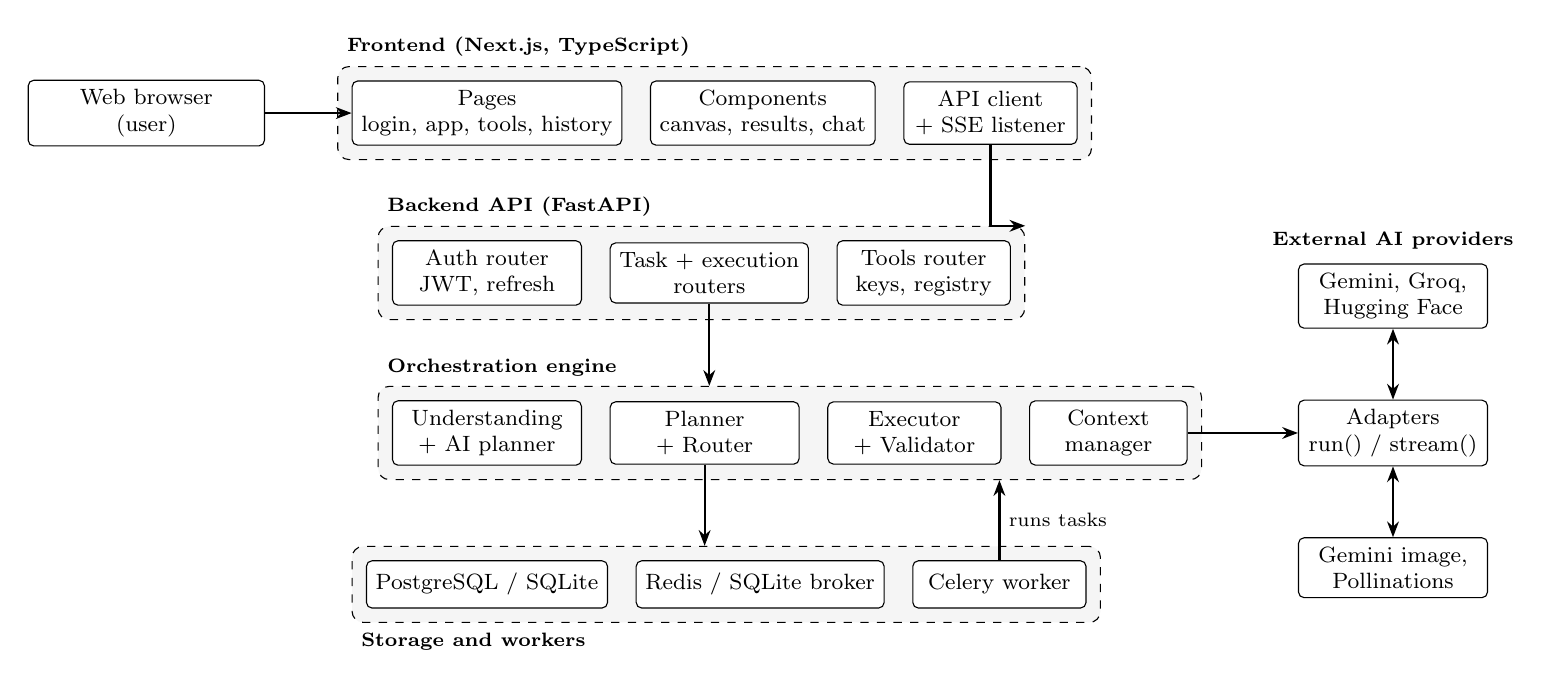
\begin{tikzpicture}[node distance=0.35cm and 0.35cm]
% client
\node[box, minimum width=3.0cm] (browser) {Web browser\\(user)};
% frontend
\node[box, right=1.1cm of browser, minimum width=2.4cm] (pages) {Pages\\login, app, tools, history};
\node[box, right=of pages, minimum width=2.4cm] (comp) {Components\\canvas, results, chat};
\node[box, right=of comp, minimum width=2.2cm] (sse) {API client\\+ SSE listener};
\begin{scope}[on background layer]
\node[layer, fit=(pages)(comp)(sse), label={[font=\scriptsize\bfseries, anchor=south west]north west:Frontend (Next.js, TypeScript)}] (fe) {};
\end{scope}
% backend api
\node[box, below=1.2cm of pages, minimum width=2.4cm] (auth) {Auth router\\JWT, refresh};
\node[box, right=of auth, minimum width=2.4cm] (taskr) {Task + execution\\routers};
\node[box, right=of taskr, minimum width=2.2cm] (toolr) {Tools router\\keys, registry};
\begin{scope}[on background layer]
\node[layer, fit=(auth)(taskr)(toolr), label={[font=\scriptsize\bfseries, anchor=south west]north west:Backend API (FastAPI)}] (api) {};
\end{scope}
% engine
\node[box, below=1.2cm of auth, minimum width=2.4cm] (und) {Understanding\\+ AI planner};
\node[box, right=of und, minimum width=2.4cm] (plan) {Planner\\+ Router};
\node[box, right=of plan, minimum width=2.2cm] (exec) {Executor\\+ Validator};
\node[box, right=of exec, minimum width=2.0cm] (ctx) {Context\\manager};
\begin{scope}[on background layer]
\node[layer, fit=(und)(plan)(exec)(ctx), label={[font=\scriptsize\bfseries, anchor=south west]north west:Orchestration engine}] (eng) {};
\end{scope}
% storage
\node[box, below=1.2cm of und, minimum width=2.4cm] (db) {PostgreSQL / SQLite};
\node[box, right=of db, minimum width=2.4cm] (redis) {Redis / SQLite broker};
\node[box, right=of redis, minimum width=2.2cm] (worker) {Celery worker};
\begin{scope}[on background layer]
\node[layer, fit=(db)(redis)(worker), label={[font=\scriptsize\bfseries, anchor=north west]south west:Storage and workers}] (st) {};
\end{scope}
% adapters + providers
\node[box, right=1.4cm of ctx, minimum width=2.4cm] (adp) {Adapters\\run() / stream()};
\node[box, above=0.9cm of adp, minimum width=2.4cm] (prov1) {Gemini, Groq,\\Hugging Face};
\node[box, below=0.9cm of adp, minimum width=2.4cm] (prov2) {Gemini image,\\Pollinations};
\node[font=\scriptsize\bfseries, above=0.05cm of prov1] {External AI providers};
\draw[arr] (browser) -- (pages);
\draw[arr] (sse) |- (api.north east);
\draw[arr] (taskr.south) -- (taskr.south |- eng.north);
\draw[arr] (plan.south) -- (plan.south |- st.north);
\draw[arr] (ctx) -- (adp);
\draw[darr] (adp) -- (prov1);
\draw[darr] (adp) -- (prov2);
\draw[arr] (worker.north) -- node[lbl, right=2pt]{runs tasks} (worker.north |- eng.south);
\end{tikzpicture}}
\caption{Layered architecture of Flow.io. The browser talks only to the frontend. The frontend talks to
the FastAPI backend over REST and SSE. The engine reaches AI providers only through adapters.}
\label{fig:system}
\end{figure*}

\subsection{Frontend Layer}
The frontend is a Next.js app written in TypeScript. It has four main pages: login and register, the
workspace, the tools page and the task history. The workspace shows the goal box, a canvas with one card
per step, a live ``Writing'' panel, the result view and the follow-up chat. The frontend does not call
any AI provider directly. It only calls the backend, which keeps API keys away from the browser.

\subsection{Backend API Layer}
The backend is a FastAPI~\cite{fastapi} service split into routers: authentication, tasks, execution,
tools, files and admin. Table~\ref{tab:api} lists the most important endpoints. All task routes check the
user's token and make sure a user can only see their own tasks.

\begin{table}[htbp]
\caption{Main REST Endpoints}
\begin{center}
\footnotesize
\begin{tabular}{@{}lp{3.7cm}@{}}
\toprule
\textbf{Endpoint} & \textbf{Purpose} \\
\midrule
POST /auth/register, /login & Create account, sign in \\
POST /auth/refresh & Get a new access token \\
POST /tasks & Create a task from a goal \\
POST /tasks/\{id\}/plan & Build the step plan \\
POST /tasks/\{id\}/execute & Start the run (returns 202) \\
GET /tasks/\{id\}/stream & Live events over SSE \\
GET /tasks/\{id\}/result & Final shaped result \\
POST /tasks/\{id\}/followup & Send a change request \\
GET /tools, POST /tools/connect & List tools, save a key \\
\bottomrule
\end{tabular}
\label{tab:api}
\end{center}
\end{table}

\subsection{Orchestration Engine}
The engine is the core of the project. It is made of six small modules, each with one job:
\begin{itemize}
\item \textbf{Understanding} reads the goal and finds the needed capabilities, counts and constraints.
\item \textbf{AI planner} asks a fast LLM to list any parts the keyword rules missed.
\item \textbf{Planner} turns capabilities into a graph of steps with dependencies.
\item \textbf{Router} scores every capable tool for each step and picks the best one.
\item \textbf{Context manager} builds the small package of facts each step is allowed to see.
\item \textbf{Executor and validator} run the steps, handle errors, check the result and repair the plan.
\end{itemize}
Fig.~\ref{fig:pipeline} shows how a request flows through these modules.

\begin{figure}[!t]
\centering
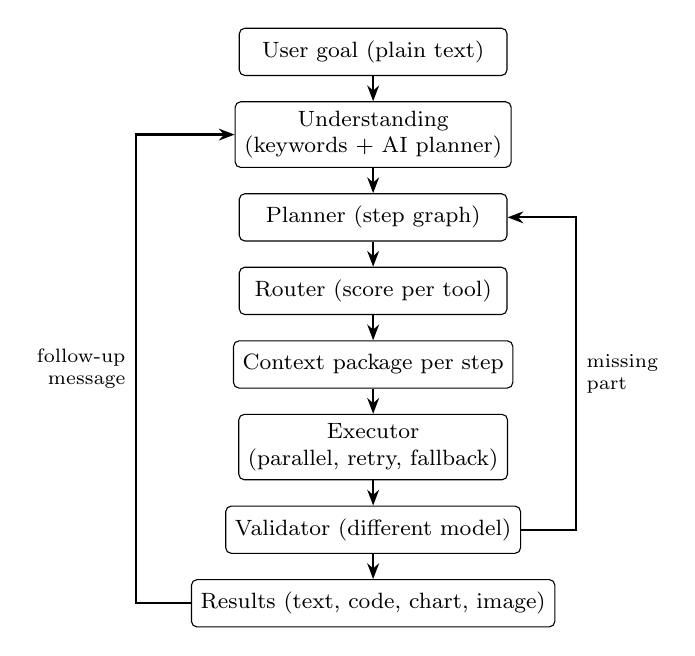
\begin{tikzpicture}[node distance=0.32cm, every node/.style={font=\footnotesize}]
\node[box, minimum width=3.4cm] (u) {User goal (plain text)};
\node[box, below=of u, minimum width=3.4cm] (a) {Understanding\\(keywords + AI planner)};
\node[box, below=of a, minimum width=3.4cm] (p) {Planner (step graph)};
\node[box, below=of p, minimum width=3.4cm] (r) {Router (score per tool)};
\node[box, below=of r, minimum width=3.4cm] (c) {Context package per step};
\node[box, below=of c, minimum width=3.4cm] (e) {Executor\\(parallel, retry, fallback)};
\node[box, below=of e, minimum width=3.4cm] (v) {Validator (different model)};
\node[box, below=of v, minimum width=3.4cm] (o) {Results (text, code, chart, image)};
\draw[arr] (u) -- (a); \draw[arr] (a) -- (p); \draw[arr] (p) -- (r);
\draw[arr] (r) -- (c); \draw[arr] (c) -- (e); \draw[arr] (e) -- (v); \draw[arr] (v) -- (o);
\draw[arr] (v.east) -- ++(0.7,0) |- node[pos=0.25, right, font=\scriptsize, align=left]{missing\\part} (p.east);
\draw[arr] (o.west) -- ++(-0.7,0) |- node[pos=0.25, left, font=\scriptsize, align=right]{follow-up\\message} (a.west);
\end{tikzpicture}
\caption{Request pipeline. The validator can send work back to the planner, and a follow-up message
starts the pipeline again with the earlier answer as context.}
\label{fig:pipeline}
\end{figure}

\subsection{Storage and Worker Layer}
All tasks, steps, runs, events and results are stored in a relational database. PostgreSQL is used in
Docker and SQLite in local development. Long runs do not happen inside the web request. Instead, the API
puts the task on a queue and returns at once with HTTP 202. A Celery~\cite{celery} worker takes the task
from the queue and runs it. Redis is the normal queue broker, and a SQLite broker is used when Redis is
not available. If the broker cannot be reached at all, the task runs in a background thread so it never
gets stuck in the ``running'' state.

\subsection{Request Lifecycle}
Fig.~\ref{fig:seq} shows the order of messages for one request. The browser creates a task, asks for a
plan, starts the run and then opens an SSE stream. The worker writes events into the database as it
works, and the stream sends them to the browser. This means the page updates live even though the work
happens in a separate process.

\begin{figure*}[t]
\centering
\resizebox{\textwidth}{!}{%
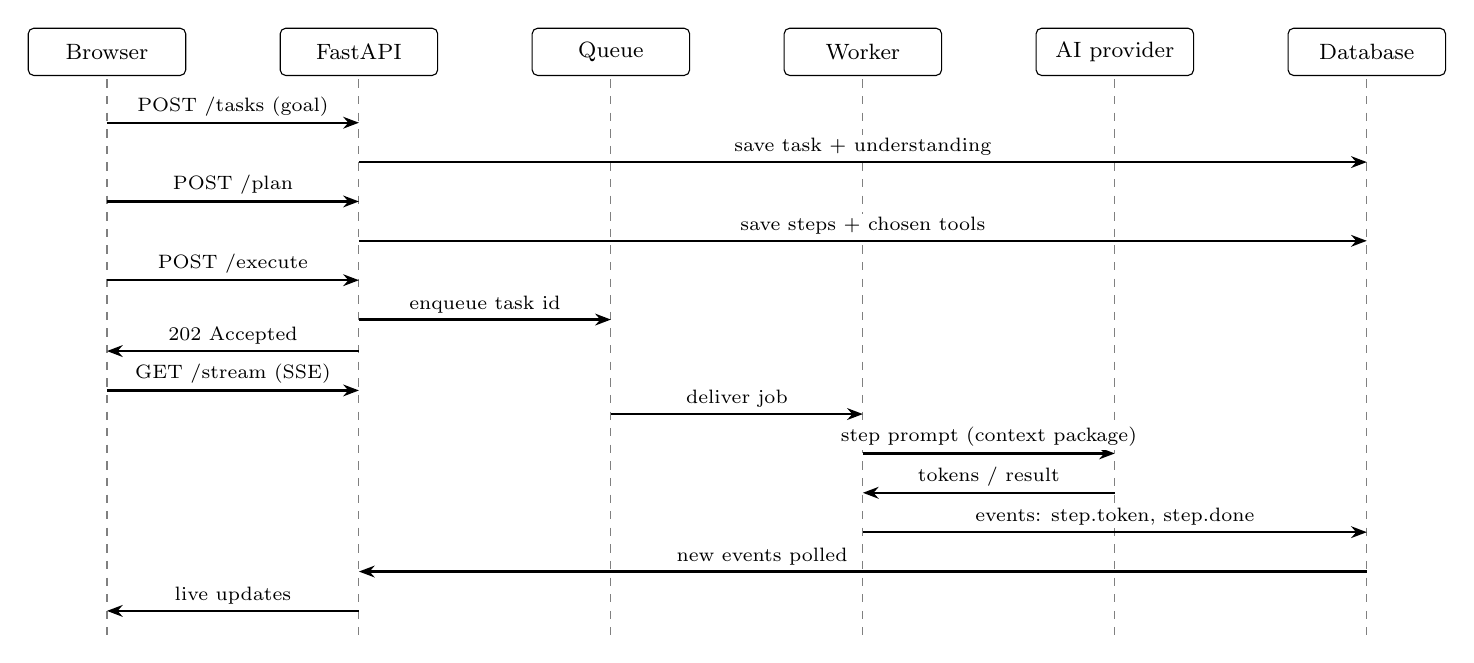
\begin{tikzpicture}[font=\footnotesize]
\foreach \x/\n/\t in {0/b/Browser, 3.2/a/FastAPI, 6.4/q/Queue, 9.6/w/Worker, 12.8/p/AI provider, 16.0/d/Database}{
  \node[box, minimum width=2.0cm] (\n) at (\x,0) {\t};
  \draw[dashed, gray] (\x,-0.35) -- (\x,-7.4);
}
\newcommand{\msg}[4]{\draw[arr] (#1,#3) -- node[lbl, above=1pt]{#4} (#2,#3);}
\msg{0}{3.2}{-0.9}{POST /tasks (goal)}
\msg{3.2}{16.0}{-1.4}{save task + understanding}
\msg{0}{3.2}{-1.9}{POST /plan}
\msg{3.2}{16.0}{-2.4}{save steps + chosen tools}
\msg{0}{3.2}{-2.9}{POST /execute}
\msg{3.2}{6.4}{-3.4}{enqueue task id}
\draw[arr] (3.2,-3.8) -- node[lbl, above=1pt]{202 Accepted} (0,-3.8);
\msg{0}{3.2}{-4.3}{GET /stream (SSE)}
\msg{6.4}{9.6}{-4.6}{deliver job}
\msg{9.6}{12.8}{-5.1}{step prompt (context package)}
\draw[arr] (12.8,-5.6) -- node[lbl, above=1pt]{tokens / result} (9.6,-5.6);
\msg{9.6}{16.0}{-6.1}{events: step.token, step.done}
\draw[arr] (16.0,-6.6) -- node[lbl, above=1pt, pos=0.6]{new events polled} (3.2,-6.6);
\draw[arr] (3.2,-7.1) -- node[lbl, above=1pt]{live updates} (0,-7.1);
\end{tikzpicture}}
\caption{Sequence of messages for one request. The run happens in the worker; the browser follows it
through the SSE stream, which reads new events from the database.}
\label{fig:seq}
\end{figure*}

\subsection{Deployment View}
Fig.~\ref{fig:deploy} shows how the system is packed for Docker Compose. Caddy acts as the public web
server and handles HTTPS. It forwards page requests to the frontend container and API requests to the
backend container. The worker container uses the same code as the backend but runs Celery instead of the
web server.

\begin{figure}[!t]
\centering
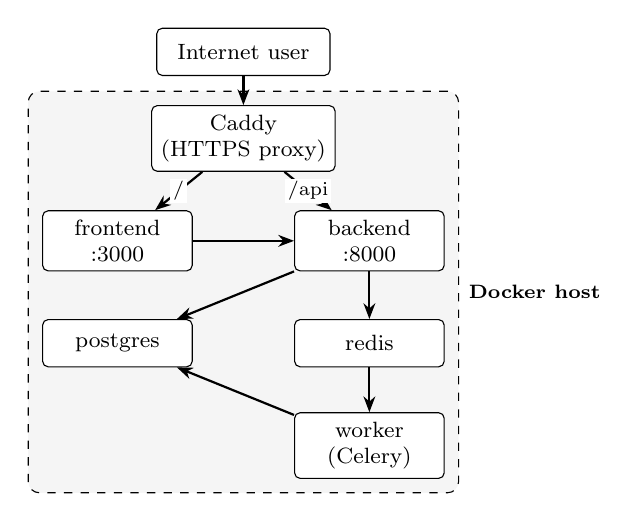
\begin{tikzpicture}[node distance=0.45cm and 0.4cm, font=\footnotesize]
\node[box, minimum width=2.2cm] (user) at (1.6,0) {Internet user};
\node[box, minimum width=2.2cm] (caddy) at (1.6,-1.1) {Caddy\\(HTTPS proxy)};
\node[box, minimum width=1.9cm] (fe) at (0,-2.4) {frontend\\:3000};
\node[box, minimum width=1.9cm] (be) at (3.2,-2.4) {backend\\:8000};
\node[box, minimum width=1.9cm] (pg) at (0,-3.7) {postgres};
\node[box, minimum width=1.9cm] (rd) at (3.2,-3.7) {redis};
\node[box, minimum width=1.9cm] (wk) at (3.2,-5.0) {worker\\(Celery)};
\draw[arr] (user) -- (caddy);
\draw[arr] (caddy) -- node[lbl]{/} (fe);
\draw[arr] (caddy) -- node[lbl]{/api} (be);
\draw[arr] (fe) -- (be);
\draw[arr] (be) -- (pg);
\draw[arr] (be) -- (rd);
\draw[arr] (rd) -- (wk);
\draw[arr] (wk) -- (pg);
\begin{scope}[on background layer]
\node[layer, fit=(caddy)(fe)(be)(wk)(pg)(rd), label={[font=\scriptsize\bfseries]right:Docker host}] {};
\end{scope}
\end{tikzpicture}
\caption{Deployment with Docker Compose. Six containers share one private network; only Caddy is open to
the internet.}
\label{fig:deploy}
\end{figure}

\section{Data Model}
The database has sixteen tables. Fig.~\ref{fig:er} shows the main ones and how they connect. A
\textit{user} owns \textit{projects} and \textit{tasks}. A task has many \textit{subtasks} (steps). Each
step can have several \textit{executions}, because a step may be retried or moved to a backup tool. Every
event that the user sees live is stored in \textit{task\_events}, and the final output is stored in
\textit{results}.

\begin{figure}[!t]
\centering
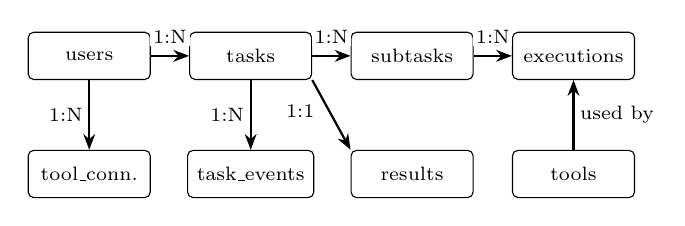
\begin{tikzpicture}[node distance=0.5cm and 0.5cm, font=\scriptsize]
\tikzset{er/.style={box, minimum width=1.55cm, font=\scriptsize}}
\node[er] (user) at (0,0) {users};
\node[er] (task) at (2.05,0) {tasks};
\node[er] (sub) at (4.1,0) {subtasks};
\node[er] (ex) at (6.15,0) {executions};
\node[er] (conn) at (0,-1.5) {tool\_conn.};
\node[er] (ev) at (2.05,-1.5) {task\_events};
\node[er] (res) at (4.1,-1.5) {results};
\node[er] (tool) at (6.15,-1.5) {tools};
\draw[arr] (user) -- node[lbl, above=3pt]{1:N} (task);
\draw[arr] (task) -- node[lbl, above=3pt]{1:N} (sub);
\draw[arr] (sub) -- node[lbl, above=3pt]{1:N} (ex);
\draw[arr] (user) -- node[lbl, left=1pt]{1:N} (conn);
\draw[arr] (task) -- node[lbl, left=1pt]{1:N} (ev);
\draw[arr] (task.south east) -- node[lbl, pos=0.45, left=4pt]{1:1} (res.north west);
\draw[arr] (tool) -- node[lbl, right=1pt]{used by} (ex);
\end{tikzpicture}
\caption{Main tables of the data model and their relations.}
\label{fig:er}
\end{figure}

The \textit{tools} table is filled from the registry file when the server starts, so the database always
matches the file. The \textit{tool\_connections} table holds each user's encrypted API keys, one row per
provider. The \textit{context\_items} and \textit{context\_transfers} tables record which facts were known
for a task and which facts were sent to each step, so a user can inspect exactly what a model saw. Other
tables store files, usage, settings, refresh tokens and an audit log.

\section{Methodology}

\subsection{Understanding the Request}
The first stage finds what the user wants. A keyword reader maps words to capabilities. For example,
``essay'', ``article'', ``story'', ``caption'' or ``email'' map to \textit{writing}, and ``photo'',
``logo'', ``poster'' or ``icon'' map to \textit{image generation}. It also reads numbers, so ``two
photos'' becomes an image count of 2 and ``500 words'' becomes a length target. Both number words and
digits are understood.

Keyword rules are fast but can miss parts of a request. So a second reader sends the request to a fast
LLM (Groq first, Gemini as backup) and asks it to return a short JSON list of every part. This AI
planner is \emph{add-only}: it can add a step the keywords missed but can never remove one. If it fails,
returns bad JSON, or takes more than 8 seconds, the keyword result is used alone. In this way the system
is never worse than the keyword rules, but it is often better. The keyword step is cached on the cleaned
goal text, so repeated requests skip the work.

\subsection{Planning the Step Graph}
The planner turns the list of capabilities into a directed graph of steps. Each step has a capability, a
title and a list of steps it depends on. Steps that do not depend on each other are put at the same level.
For example, writing an essay and making a picture both depend only on the goal, so they run together. A
step that needs research comes after the research step. A validation step is always added at the end and
depends on all the others.

\subsection{Score-Based Routing}
Each model is described in a registry file (\texttt{tools.json}) by its capabilities, speed class, cost
class, context window, provider and whether it needs a key. The router code does not contain any
provider names. It only reads this metadata. For a step with capability $k$, the router gives each
capable tool $t$ the score:
\begin{equation}
S_t = \frac{w_q Q_t + w_c C_t + w_s V_t}{w_q + w_c + w_s} + B_t
\label{eq:score}
\end{equation}
where $Q_t$, $C_t$ and $V_t$ are the quality, cost and speed values of the tool, and $(w_q, w_c, w_s)$
are weights that depend on the type of step (Table~\ref{tab:weights}). Speed values are 1.0, 0.6 and 0.2
for fast, mid and slow. Cost values are 1.0, 0.6 and 0.2 for low, mid and high, so a cheaper tool scores
higher on cost. Quality is taken from the cost class (1.0, 0.7 and 0.4 for high, mid and low), based on
the guess that a costlier model is stronger.

\begin{table}[htbp]
\caption{Routing Weights per Step Type}
\begin{center}
\begin{tabular}{@{}lccc@{}}
\toprule
\textbf{Step type} & \textbf{Quality} & \textbf{Cost} & \textbf{Speed} \\
\midrule
Writing, reasoning & 0.60 & 0.20 & 0.20 \\
Code generation & 0.65 & 0.20 & 0.15 \\
Long documents & 0.50 & 0.25 & 0.25 \\
Image generation & 0.60 & 0.25 & 0.15 \\
Validation, web research & 0.30 & 0.30 & 0.40 \\
File processing & 0.20 & 0.45 & 0.35 \\
Code execution & 0.20 & 0.40 & 0.40 \\
\bottomrule
\end{tabular}
\label{tab:weights}
\end{center}
\end{table}

The term $B_t$ adds the practical adjustments listed in Table~\ref{tab:bonus}. Before scoring, a tool is
removed completely if the text the step must read is more than 80\% of its context window. The user can
also choose a priority (balanced, quality, cheap or fast), which doubles the matching weight.

\begin{table}[htbp]
\caption{Score Adjustments ($B_t$)}
\begin{center}
\begin{tabular}{@{}lc@{}}
\toprule
\textbf{Condition} & \textbf{Change} \\
\midrule
Key saved, or no key needed & $+0.25$ \\
Key needed but not saved (live mode) & $-0.85$ \\
Free space left in context window & up to $+0.10$ \\
Specialist tool (at most 2 capabilities) & $+0.10$ \\
Fast step: speed and low-cost bonus & up to $+0.20$ \\
Same tool that wrote the answer (check) & $-0.20$ \\
Step needs files or images, tool lacks it & $-0.30$ \\
\bottomrule
\end{tabular}
\label{tab:bonus}
\end{center}
\end{table}

Algorithm~\ref{alg:route} gives the full procedure. The tool with the highest score runs the step. The
rest are kept in score order as backups. Ties are broken by tool name so the result is always the same
for the same input. The router also returns a confidence value based on the gap between the first and
second scores, and a list of plain reasons such as ``Fast'', ``Low cost'' or ``Different from the tool
that wrote the result''. These reasons are shown on each step card.

\begin{algorithm}[htbp]
\caption{Per-Step Tool Routing}
\label{alg:route}
\footnotesize
\begin{algorithmic}[1]
\Require capability $k$, tools $T$, saved providers $P$, tokens $n$
\State $C \gets \{t \in T : t \text{ available and } k \in t.\text{caps}\}$
\If{$C = \emptyset$} \Return no tool, ``cannot do $k$ yet'' \EndIf
\State $(w_q,w_c,w_s) \gets \text{PROFILE}[k] \times \text{PRIORITY}$
\ForAll{$t \in C$}
  \If{$n > 0.8 \cdot t.\text{window}$} \textbf{continue} \EndIf
  \State $S_t \gets$ weighted mean of $Q_t, C_t, V_t$ \Comment{Eq.~(\ref{eq:score})}
  \State add context, specialist and fast-step bonuses
  \If{$t$ needs a key and $t.\text{provider} \notin P$} $S_t \gets S_t - 0.85$
  \Else{} $S_t \gets S_t + 0.25$ \EndIf
  \If{$t$ wrote the answer being checked} $S_t \gets S_t - 0.2$ \EndIf
\EndFor
\State sort tools by $(-S_t, t.\text{id})$
\State \Return first tool, others as ordered backups, reasons
\end{algorithmic}
\end{algorithm}

Fig.~\ref{fig:scores} shows the real scores the router gives for a writing step when Gemini and Groq keys
are saved but Hugging Face and Anthropic keys are not. The three tools with keys score close to 1.0.
Tools without a key fall below zero, so they are used only if everything else fails.

\begin{figure}[!t]
\centering
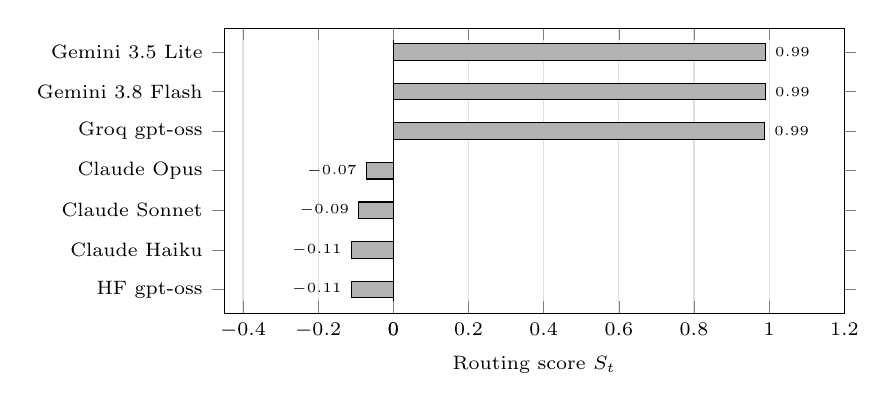
\begin{tikzpicture}
\begin{axis}[
  xbar, width=0.78\columnwidth, height=5.2cm,
  xmin=-0.45, xmax=1.2,
  /pgf/number format/.cd, fixed, precision=2, /pgfplots/.cd,
  symbolic y coords={HF gpt-oss,Claude Haiku,Claude Sonnet,Claude Opus,Groq gpt-oss,Gemini 3.8 Flash,Gemini 3.5 Lite},
  ytick=data, yticklabel style={font=\scriptsize},
  xticklabel style={font=\scriptsize},
  xlabel={Routing score $S_t$}, xlabel style={font=\scriptsize},
  nodes near coords, nodes near coords style={font=\tiny},
  bar width=6pt, xmajorgrids, grid style={gray!25},
  extra x ticks={0}, extra x tick style={grid=major, grid style={black}},
]
\addplot[fill=gray!60] coordinates {
 (-0.112,HF gpt-oss) (-0.112,Claude Haiku) (-0.092,Claude Sonnet) (-0.072,Claude Opus)
 (0.988,Groq gpt-oss) (0.99,Gemini 3.8 Flash) (0.99,Gemini 3.5 Lite)};
\end{axis}
\end{tikzpicture}
\caption{Router scores for a writing step (2,000 tokens of context) with Gemini and Groq keys saved.
Values are taken from running the router code on the real registry.}
\label{fig:scores}
\end{figure}

\subsection{Context Management}
Sending the full history to every model wastes tokens and can confuse the model. The context manager
solves this with a policy table. For each step type it lists which kinds of facts the step may see, such
as the objective, requirements, constraints, decisions, research, earlier outputs and files. For example,
an image step sees the objective, requirements, constraints and decisions, but not long research notes.
A validation step sees the objective, requirements and the outputs it must check. Facts are added in a
fixed priority order until the token budget of the chosen tool is reached. Every package that is sent is
recorded, so the user can open a step and see what was passed and what was held back.

For image steps the prompt is built only from the picture-related parts of the request, plus any recent
change requests from the chat. This stops the image model from receiving text like ``write a 500 word
essay'', which it cannot use.

\subsection{Execution, Retries and Fallback}
The executor runs the plan level by level. All steps in one level are started in parallel threads, and
the next level starts only when the current one is finished. Fig.~\ref{fig:state} shows the states a
step can go through.

\begin{figure}[!t]
\centering
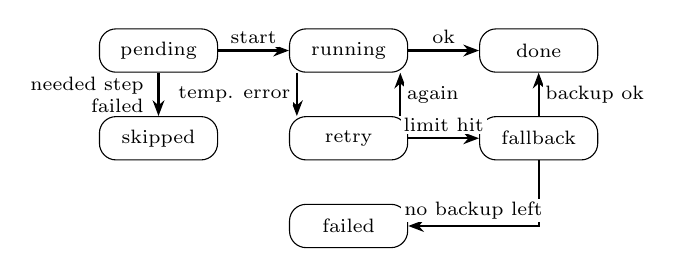
\begin{tikzpicture}[node distance=0.55cm and 0.9cm, font=\scriptsize,
  st/.style={draw, rounded corners=6pt, minimum width=1.5cm, minimum height=0.55cm, align=center, fill=white}]
\node[st] (pen) {pending};
\node[st, right=of pen] (run) {running};
\node[st, right=of run] (done) {done};
\node[st, below=of run] (retry) {retry};
\node[st, below=of done] (fb) {fallback};
\node[st, below=of retry] (fail) {failed};
\node[st, below=of pen] (skip) {skipped};
\draw[arr] (pen) -- node[lbl, above=1pt]{start} (run);
\draw[arr] (run) -- node[lbl, above=1pt]{ok} (done);
\draw[arr] (run.south west) ++(0.1,0) -- node[lbl, left=1pt]{temp. error} ($(retry.north west)+(0.1,0)$);
\draw[arr] ($(retry.north east)-(0.1,0)$) -- node[lbl, right=1pt]{again} ($(run.south east)-(0.1,0)$);
\draw[arr] (retry) -- node[lbl, above=1pt]{limit hit} (fb);
\draw[arr] (fb) -- node[lbl, right=1pt]{backup ok} (done);
\draw[arr] (fb) |- node[lbl, pos=0.75, above=1pt]{no backup left} (fail);
\draw[arr] (pen) -- node[lbl, left=4pt, align=right]{needed step\\failed} (skip);
\end{tikzpicture}
\caption{States of one step during execution.}
\label{fig:state}
\end{figure}

Each provider call has a time limit of 120 seconds. If a provider returns a temporary error, such as a
timeout, a network error or HTTP 429 (too many requests), the step is retried up to 2 times with
exponential backoff of 0.5 and then 1 second. If it still fails, the next tool in the backup list takes
over and the user sees a ``fallback'' event. If no backup is left, the step fails with a clear message,
and steps that needed it are skipped. For images, if Gemini refuses the request, for example because a
free key has no image quota, the system falls back to the free Pollinations service. The real reason
from Google is kept in the error message so the user knows what happened.

\subsection{Live Streaming}
Users feel a system is slow when they stare at a blank screen. To fix this, text steps stream their answer
token by token. The adapter's \texttt{stream()} method reads the provider's server-sent stream and yields
small pieces of text. The executor groups them and stores them as \texttt{step.token} events. The
frontend shows them in a ``Writing'' panel with a typing cursor. After the stream ends, the full
\texttt{run()} result is used as the final answer, so a broken stream only loses the preview and never the
answer. Other events, such as \texttt{step.started}, \texttt{step.retry}, \texttt{step.fallback} and
\texttt{task.done}, update the step cards in real time.

\subsection{Validation and Self-Repair}
The last step asks a different model to check the result against the original goal. Because of the
$-0.2$ penalty in Table~\ref{tab:bonus}, the model that wrote the answer is not chosen to grade it when
another good choice exists. The check returns pass, fail or unknown, with a short reason.

The system then reads that reason, as shown in Fig.~\ref{fig:repair}. If it says a whole part is
missing, for example ``the essay is missing'', the matching capability is found, a new step is added to
the plan and run. If the reason names a weak part, only that step is run again with the reason added to
its context. To stop endless loops, only one repair round is allowed per run.

\begin{figure}[!t]
\centering
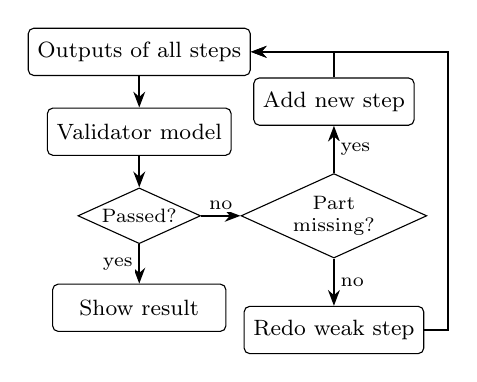
\begin{tikzpicture}[node distance=0.4cm and 0.5cm, font=\scriptsize]
\node[box, minimum width=2.2cm] (out) {Outputs of all steps};
\node[box, below=of out, minimum width=2.2cm] (chk) {Validator model};
\node[draw, diamond, aspect=2.2, inner sep=1pt, below=of chk, font=\scriptsize] (dec) {Passed?};
\node[box, below=0.5cm of dec, minimum width=2.2cm] (fin) {Show result};
\node[draw, diamond, aspect=2.2, inner sep=1pt, right=0.5cm of dec, font=\scriptsize, align=center] (miss) {Part\\missing?};
\node[box, above=0.6cm of miss, minimum width=1.9cm] (add) {Add new step};
\node[box, below=0.6cm of miss, minimum width=1.9cm] (redo) {Redo weak step};
\draw[arr] (out) -- (chk); \draw[arr] (chk) -- (dec);
\draw[arr] (dec) -- node[lbl, left=1pt]{yes} (fin);
\draw[arr] (dec) -- node[lbl, above=1pt]{no} (miss);
\draw[arr] (miss) -- node[lbl, right=1pt]{yes} (add);
\draw[arr] (miss) -- node[lbl, right=1pt]{no} (redo);
\draw[arr] (add) |- (out);
\draw[arr] (redo.east) -- ++(0.3,0) |- (out.east);
\end{tikzpicture}
\caption{Validation and repair loop (at most one repair round per run).}
\label{fig:repair}
\end{figure}

\subsection{Follow-Up Chat}
After a result is shown, the user can type a change in a chat box under it, such as ``make the background
blue'' or ``now write an Instagram caption''. The message is saved with the task and marked as a change
request. The task then runs again with the first goal, all earlier changes and the previous answer in its
context. If the message asks for new work, the same understanding rules find the new capability and a
new step is added before the check. Numbers in the message, such as ``make it 3 photos'', update the
saved counts. The chat history stays with the task, so it is still there when the user opens the task
later.

\section{Implementation}

\subsection{Technology Stack}
Table~\ref{tab:stack} lists the main technologies. The backend has about 2,850 lines of Python, and the
frontend has about 2,300 lines of TypeScript.

\begin{table}[htbp]
\caption{Technology Stack}
\begin{center}
\footnotesize
\begin{tabular}{@{}ll@{}}
\toprule
\textbf{Part} & \textbf{Technology} \\
\midrule
Frontend & Next.js, React, TypeScript \\
Backend API & Python, FastAPI, Pydantic \\
Database & PostgreSQL / SQLite, SQLAlchemy \\
Migrations & Alembic \\
Task queue & Celery with Redis (or SQLite broker) \\
Live updates & Server-Sent Events \\
HTTP client & httpx \\
Security & JWT, Argon2, Fernet, rate limits \\
Testing & pytest, TypeScript compiler \\
Deployment & Docker Compose, Caddy \\
\bottomrule
\end{tabular}
\label{tab:stack}
\end{center}
\end{table}

\subsection{Tool Registry and Adapters}
The registry holds 14 tools, shown in Table~\ref{tab:tools}. Each provider is wrapped in an adapter that
follows the same small interface: \texttt{run(package)} returns the full result, and \texttt{stream(package)}
yields text pieces. A base class gives a default \texttt{stream()} that simply calls \texttt{run()}, so
adapters that cannot stream still work. Adding a new provider means writing one adapter class and adding
one entry to the registry file. No other part of the code changes.

\begin{table}[htbp]
\caption{Tools in the Registry}
\begin{center}
\scriptsize
\resizebox{\columnwidth}{!}{%
\begin{tabular}{@{}llll@{}}
\toprule
\textbf{Tool} & \textbf{Main jobs} & \textbf{Speed/Cost} & \textbf{Context} \\
\midrule
Gemini 3.8 Flash & text, code, check & fast/low & 1M \\
Gemini 3.5 Flash Lite & text, check & fast/low & 1M \\
Gemini search & web research & fast/low & 1M \\
Groq gpt-oss-120b & text, code, check & fast/low & 131K \\
HF gpt-oss-120b & text, code, check & fast/low & 131K \\
Gemini image & images & mid/low & -- \\
Pollinations & images (free) & mid/low & -- \\
Claude Opus / Sonnet & text, code, check & slow-mid/high-mid & 128K \\
Claude Haiku & text, check & fast/low & 128K \\
Brave search & web research & fast/low & -- \\
OpenAI image & images & mid/mid & -- \\
Local image, sandbox & planned & -- & -- \\
\bottomrule
\end{tabular}}
\label{tab:tools}
\end{center}
\end{table}

In the current build, the user mainly uses Gemini and Groq keys. Hugging Face is used as an extra online
chat model and acts as a backup when its key is saved. It is called through Hugging Face's router API,
and no model runs on the user's own machine.

\subsection{User Interface}
The interface was designed to be clean and calm. Each step is shown as a card with its title, its chosen
tool and the reasons for the choice. A running card pulses, and a finished card pops once. Clicking a
card opens a side panel with the context package, the raw output, and every attempt. The result view
adapts to the output type: text is shown as formatted writing, code is shown in file tabs with a copy
button, numbers can be shown as a bar chart, and images are shown in a gallery. Results can be exported
as a Markdown file.

Page changes use a short fade with a thin progress bar at the top, and buttons give a ripple on click. All
motion is turned off when the operating system's ``reduce motion'' setting is on. The layout works on
small screens without sideways scrolling.

\subsection{Demo Mode}
A demo mode runs the full pipeline with no API keys. A demo adapter returns placeholder text and images,
and every output is clearly marked ``Simulated''. This was useful for building the interface before keys
were added, and it lets anyone try the flow without paying for an API.

\section{Security Design}
Since users save their own paid API keys, security was treated as a main requirement:
\begin{itemize}
\item \textbf{Passwords} are hashed with Argon2. A dummy hash is checked when an email is unknown, so an
attacker cannot tell real accounts apart by response time.
\item \textbf{Sessions} use short-lived JWT access tokens and refresh tokens that last 14 days. Refresh
tokens are stored only as SHA-256 hashes and can be revoked on logout.
\item \textbf{API keys} are encrypted with Fernet before they are saved and are never sent back to the
browser. Only the backend decrypts them, right before a provider call.
\item \textbf{Rate limits} protect sensitive routes, for example 10 login tries and 10 key saves per
minute for each IP address, and 20 runs per minute.
\item \textbf{Access control} checks that each task belongs to the user asking for it.
\item \textbf{Network}: in deployment only the Caddy proxy is public; the database, Redis and worker are
on a private network.
\end{itemize}

\section{Testing and Results}

\subsection{Automated Tests}
The backend has 95 test functions written with pytest. Some are run with several inputs, giving 101 test
cases in total, and all of them pass. Fig.~\ref{fig:tests} shows how the test functions are spread over
the main areas of the system. The tests use fake provider responses, so they run in about four seconds
and do not need real keys or internet. The frontend passes TypeScript type checking and a production
build.

\begin{figure}[!t]
\centering
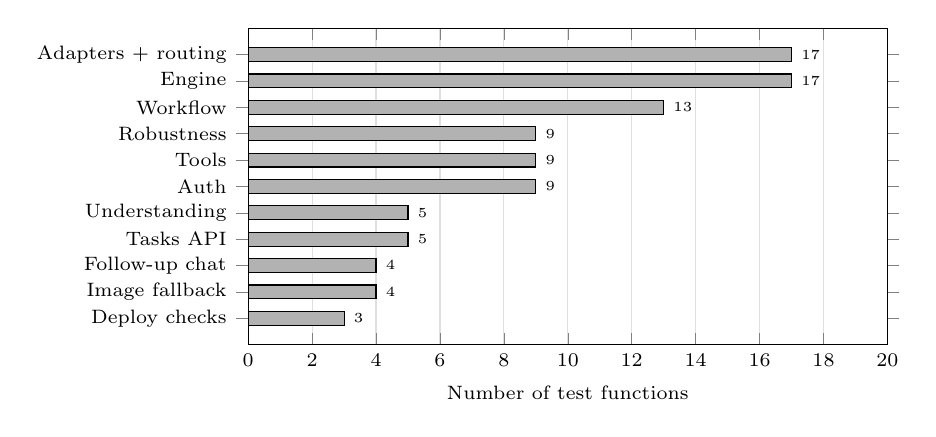
\begin{tikzpicture}
\begin{axis}[
  xbar, width=0.80\columnwidth, height=5.6cm, xmin=0, xmax=20,
  symbolic y coords={Deploy checks,Image fallback,Follow-up chat,Tasks API,Understanding,Auth,Tools,Robustness,Workflow,Engine,Adapters + routing},
  ytick=data, yticklabel style={font=\scriptsize}, xticklabel style={font=\scriptsize},
  xlabel={Number of test functions}, xlabel style={font=\scriptsize},
  nodes near coords, nodes near coords style={font=\tiny},
  bar width=5pt, xmajorgrids, grid style={gray!25},
]
\addplot[fill=gray!60] coordinates {
 (3,Deploy checks) (4,Image fallback) (4,Follow-up chat) (5,Tasks API) (5,Understanding)
 (9,Auth) (9,Tools) (9,Robustness) (13,Workflow) (17,Engine) (17,Adapters + routing)};
\end{axis}
\end{tikzpicture}
\caption{Test functions per area of the system (95 functions, 101 cases).}
\label{fig:tests}
\end{figure}

Table~\ref{tab:testcov} lists some of the most important behaviours the tests check.

\begin{table}[htbp]
\caption{Key Behaviours Covered by Tests}
\begin{center}
\footnotesize
\begin{tabular}{@{}lp{4.6cm}@{}}
\toprule
\textbf{Area} & \textbf{What is checked} \\
\midrule
Routing & Keyed tool wins, oversize context is skipped, checker differs from writer \\
Robustness & Retry on timeout and 429, fallback to backup, broker-down thread fallback \\
Parallel & Independent steps run at the same time \\
Understanding & Essay + 2 photos gives writing and image steps with counts \\
Repair & ``Essay missing'' adds a writing step \\
Follow-up & Change request reruns task with history \\
Security & Login rate limit, token refresh, user isolation \\
Deploy & Migrations build every table on an empty database \\
\bottomrule
\end{tabular}
\label{tab:testcov}
\end{center}
\end{table}

\subsection{End-to-End Checks}
Beyond unit tests, several checks were done on the running system. A real Celery worker process picked up
a task from a SQLite broker and finished it. The free image service was called for real and returned two
different car pictures for one request. The Alembic migrations were run on a fresh database and compared
with the models to make sure no table or column was missing.

\subsection{Case Study}
Table~\ref{tab:case} shows one real request before and after the improvements to understanding and
validation: \textit{``write a 500 words essay on cars and generate two photos''}.

\begin{table}[htbp]
\caption{Case Study: Essay and Two Photos}
\begin{center}
\footnotesize
\begin{tabular}{@{}lll@{}}
\toprule
\textbf{Item} & \textbf{Before} & \textbf{After} \\
\midrule
Steps planned & Image, Check & Writing + Image, Check \\
Essay produced & No & Yes (500-word target) \\
Photos produced & 1 & 2, different \\
Writing and image & -- & Run in parallel \\
Check finds a gap & Redid image & Adds missing step \\
``Where is the essay?'' & Redrew image & Adds the essay \\
\bottomrule
\end{tabular}
\label{tab:case}
\end{center}
\end{table}

In the first version, the word ``essay'' was not in the keyword list, so only the image step was planned.
The check step noticed that the essay was missing but had no way to add it, so it redid the image. After
the changes, all parts of the request were planned, the essay and images ran at the same time, and the
two image calls produced two different pictures. This case showed why both the AI planner and the repair
loop are needed: either one alone would have caught this error, and together they make it much less
likely that a part of the request is silently dropped.

\subsection{Discussion of Speed}
Early users found the app slow because each step waited for the full model answer. Streaming does not
change the total time much, but the first words now appear as soon as the model starts writing, which
makes the app feel much faster. Running independent steps in parallel cuts the real total time, because
the writing step and the image step no longer wait for each other. Sending the check step to the
fastest cheap tool also shortens the end of each run. These gains have not yet been measured with exact
timings.

\section{Limitations and Future Work}

\subsection{Current Limitations}
\begin{itemize}
\item \textbf{Hand-set quality.} Quality values are guessed from the cost class and are not measured.
Gemini and Groq have the same labels, so the router treats them as almost equal, and ties are decided by
name. This is visible in Fig.~\ref{fig:scores}.
\item \textbf{Image limits.} A free Gemini key has no image quota. The free fallback service adds a small
watermark, handles text inside images poorly, and allows one picture every 45 seconds.
\item \textbf{Mocked tests.} The AI planner and most adapters were tested against fake providers, not
live ones.
\item \textbf{Deployment.} The Docker images and a public deployment have not yet been checked on a real
server.
\item \textbf{Image edits.} A follow-up change to an image draws a new picture. The old picture is not
edited, so details may change.
\item \textbf{No user study.} The system has not yet been tested with a group of real users.
\end{itemize}

\subsection{Future Work}
The most important next step is measured routing. The system will record the time, token use and check
result of every model call. These numbers will replace the hand-set labels in (\ref{eq:score}), so the
router learns which model is really faster and better for each step type. A simple moving average per
tool and step type would be enough to start.

Other planned work includes:
\begin{itemize}
\item showing the plan to the user before it runs, so they can edit it;
\item more image providers, and real image editing for follow-up changes;
\item a safe sandbox to run generated code;
\item cost tracking and a spending limit per task;
\item a small user study to measure time saved compared with switching apps by hand.
\end{itemize}

\section{Conclusion}
Flow.io shows that one interface can hide many AI models from the user. A request is split into steps.
Each step is given to a suitable model by a simple, explainable scoring rule, and gets only the context it
needs. Independent steps run in parallel, errors are handled by retries and backups, and a second model
checks the result and can trigger a repair. Because all model details live in a registry file and every
provider sits behind the same adapter interface, new providers can be added with very little code. The
system works end to end today and is backed by an automated test suite. Its next step is to replace
estimated model labels with measured performance, so that the choice of model is based on real results.

\section*{Acknowledgment}
The author thanks the guide and the department for their support during this project.

\begin{thebibliography}{00}
\bibitem{hugginggpt} Y. Shen, K. Song, X. Tan, D. Li, W. Lu, and Y. Zhuang, ``HuggingGPT: Solving AI
tasks with ChatGPT and its friends in Hugging Face,'' in \textit{Advances in Neural Information
Processing Systems (NeurIPS)}, 2023.
\bibitem{react} S. Yao, J. Zhao, D. Yu, N. Du, I. Shafran, K. Narasimhan, and Y. Cao, ``ReAct:
Synergizing reasoning and acting in language models,'' in \textit{Proc. Int. Conf. Learning
Representations (ICLR)}, 2023.
\bibitem{toolformer} T. Schick \textit{et al.}, ``Toolformer: Language models can teach themselves to use
tools,'' in \textit{Advances in Neural Information Processing Systems (NeurIPS)}, 2023.
\bibitem{autogen} Q. Wu \textit{et al.}, ``AutoGen: Enabling next-gen LLM applications via multi-agent
conversation,'' arXiv:2308.08155, 2023.
\bibitem{langchain} H. Chase, ``LangChain,'' 2022. [Online]. Available:
\url{https://github.com/langchain-ai/langchain}
\bibitem{frugalgpt} L. Chen, M. Zaharia, and J. Zou, ``FrugalGPT: How to use large language models while
reducing cost and improving performance,'' arXiv:2305.05176, 2023.
\bibitem{routellm} I. Ong \textit{et al.}, ``RouteLLM: Learning to route LLMs with preference data,''
arXiv:2406.18665, 2024.
\bibitem{fastapi} S. Ram\'irez, ``FastAPI.'' [Online]. Available: \url{https://fastapi.tiangolo.com}
\bibitem{celery} Celery Project, ``Celery: Distributed task queue.'' [Online]. Available:
\url{https://docs.celeryq.dev}
\end{thebibliography}

\end{document}
